\documentclass[aps,pra,reprint,superscriptaddress,amsmath,amssymb,longbibliography]{revtex4-2}
\usepackage{graphicx}
\usepackage{tikz}
\usepackage{xcolor}
\usepackage{amsthm}
\usepackage[hidelinks]{hyperref}
\newcommand{\ket}[1]{|#1\rangle}
\newcommand{\bra}[1]{\langle#1|}
\newcommand{\AME}{\mathrm{AME}}
\newcommand{\todo}[1]{\textcolor{red}{[#1]}}
\theoremstyle{plain}
\newtheorem{proposition}{Proposition}
\newtheorem{lemma}{Lemma}
\newtheorem{theorem}{Theorem}

\begin{document}
% Working title.  Alternatives:
%   "Euler's thirty-six officers need no complex numbers"
%   "Real absolutely maximally entangled states of four quhexes: families and classification"
\title{Real absolutely maximally entangled states of four six-level systems}
\author{Palash Pandya}
\affiliation{\todo{affiliation}}
\date{\today}

\begin{abstract}
Absolutely maximally entangled states of four six-level systems, AME$(4,6)$, are the quantum solutions of Euler's
problem of the thirty-six officers.  All solutions found so far have complex coefficients, and it has been
conjectured that no real orthogonal two-unitary matrix of order $36$ exists.  We give real AME$(4,6)$ states with
$60$ non-zero coefficients in $\{\pm1,\sqrt2\}/\sqrt{72}$, together with a proof that can be checked by hand.
They lie in the $-1$ eigenspace of an order-four local symmetry, and on their support the AME conditions become linear.
This yields two families of AME$(4,6)$ states in closed form: a ten-parameter family that contains two-unitary
complex weighing matrices with uniform amplitudes, and an eleven-parameter family on $60$ basis states.  The real
states sit where the two families meet.  On this support there are $2048$ real AME states up to local phases.  They
are isolated, and they fall into exactly eight classes under local unitaries and permutations of the parties; we
certify the separation of the classes with interval arithmetic.  Code and data are public.
\end{abstract}
\maketitle

% =========================================================================================================
\section{Introduction}

A pure state of $N$ parties with $d$ levels each is absolutely maximally entangled, AME$(N,d)$, if every reduction
to $\lfloor N/2\rfloor$ parties is maximally mixed~\cite{Helwig2012,GALRZ15}.  Such states are perfect tensors; they
underlie quantum secret sharing~\cite{Helwig2012}, holographic codes~\cite{PYHP2015} and dual-unitary
circuits~\cite{BKP2019}.  For four parties, writing $U_{(ij),(kl)}=d\,\psi_{ijkl}$, the state is AME if and only if
$U$ is \emph{two-unitary}: $U$, its realignment $U^R$ and its partial transpose $U^\Gamma$ are all
unitary~\cite{GALRZ15}.  Up to permutations of rows and columns, these three matrices are the reshapings of
$d\,\psi$ along the three bipartitions $12|34$, $13|24$ and $14|23$.

A pair of orthogonal Latin squares of order $d$ gives a two-unitary permutation matrix.  Such pairs exist for every
$d\ge3$ except $d=6$~\cite{BSP1960}: Euler's problem of the $36$ officers has no
solution~\cite{Euler1782,Tarry1900}.  AME$(4,2)$ states do not exist at all~\cite{HS2000}.  An AME$(4,6)$ state, a
quantum solution of Euler's problem, was found by Rather \emph{et al.}~\cite{RBB22}.  Further solutions include
continuous families obtained from it~\cite{RRKL23}, two-unitary complex Hadamard matrices~\cite{BZ24}, constructions
from biunimodular vectors~\cite{Rat24} and hand-made solutions~\cite{GG25}.  No stabilizer AME$(4,6)$ state
exists~\cite{WMBA26}, and quantum solutions are necessarily entangled~\cite{BS26}.

All of these solutions are complex.  In the Supplemental Material of Ref.~\cite{RBB22} the authors write:
``Further numerical results suggest that any 2-unitary matrix $U_{36}$ has complex entries.  Therefore, it is
tempting to conjecture that there exists no solution in the set $O(36)$ of orthogonal matrices of this size.''  A
recent review lists the question as open problem (T2)~\cite{RBRLZ26}: ``Is there an AME(4,6) state with real
coefficients? Equivalently, is there an orthogonal 2-unitary matrix of order 36?''

We answer this question in the affirmative.  With the permutation solutions for $d\neq2,6$, it follows that a real
AME$(4,d)$ state exists if and only if $d\ge3$, exactly when a complex one does.  Our results are the following.
(i)~An explicit real AME$(4,6)$ state with $60$ non-zero coefficients, the sparsest AME$(4,6)$ state we know of,
whose two-unitaries are direct sums of $1\times1$ and $2\times2$ blocks (Sec.~\ref{sec:state}).
(ii)~Its origin: it lies in the $-1$ eigenspace of the local symmetry
$u^{\otimes4}$, $u=\mathrm{diag}(i,-1,-1,-i,-i,-i)$, and on its support the AME conditions are linear
(Sec.~\ref{sec:symmetry}).
(iii)~Two continuous families of AME$(4,6)$ states in closed form that meet at the real state; one contains
two-unitary complex weighing matrices (Sec.~\ref{sec:families}).
(iv)~A complete classification of the real AME states on this support: $2048$ states, all isolated, in exactly
eight classes under local unitaries and party permutations (Sec.~\ref{sec:real}).
All statements are verified by self-contained scripts~\cite{repo}.

% =========================================================================================================
\section{A real AME(4,6) state}\label{sec:state}

Label the levels of each party by $0,\dots,5$ and let
\begin{widetext}
% generated by paper/make_state_table.py from data/psi_terms.json -- do not edit
\begin{center}
\renewcommand{\arraystretch}{1.4}\setlength{\tabcolsep}{8pt}
\begin{tabular}{c|cccccc}
$\ket{\phi_{ab}}$ & $b=0$ & $b=1$ & $b=2$ & $b=3$ & $b=4$ & $b=5$\\\hline
$a=0$ & $-\ket{12}+\ket{21}$ & $-\ket{02}+\ket{20}$ & $-\ket{01}+\ket{10}$ & \cellcolor{gray!18}$\sqrt2\,\ket{44}$ & \cellcolor{gray!18}$\sqrt2\,\ket{55}$ & \cellcolor{gray!18}$\sqrt2\,\ket{33}$\\
$a=1$ & $-\ket{01}-\ket{10}$ & $\ket{00}+\ket{54}$ & $\ket{35}+\ket{43}$ & $-\ket{15}-\ket{32}$ & $-\ket{23}+\ket{41}$ & $-\ket{24}+\ket{52}$\\
$a=2$ & $\ket{02}+\ket{20}$ & $-\ket{35}+\ket{43}$ & $\ket{00}-\ket{54}$ & $-\ket{25}+\ket{31}$ & $-\ket{13}+\ket{42}$ & $\ket{14}+\ket{51}$\\
$a=3$ & \cellcolor{gray!18}$\sqrt2\,\ket{34}$ & $-\ket{23}-\ket{41}$ & $\ket{13}+\ket{42}$ & \cellcolor{gray!18}$\sqrt2\,\ket{50}$ & $-\ket{11}+\ket{22}$ & \cellcolor{gray!18}$\sqrt2\,\ket{05}$\\
$a=4$ & \cellcolor{gray!18}$\sqrt2\,\ket{53}$ & $\ket{15}-\ket{32}$ & $\ket{25}+\ket{31}$ & $\ket{11}+\ket{22}$ & \cellcolor{gray!18}$\sqrt2\,\ket{04}$ & \cellcolor{gray!18}$\sqrt2\,\ket{40}$\\
$a=5$ & \cellcolor{gray!18}$\sqrt2\,\ket{45}$ & $-\ket{14}+\ket{51}$ & $\ket{24}+\ket{52}$ & \cellcolor{gray!18}$\sqrt2\,\ket{03}$ & \cellcolor{gray!18}$\sqrt2\,\ket{30}$ & $\ket{12}+\ket{21}$\\
\end{tabular}
\end{center}

\end{widetext}
The $60$ basis states fall into two sets.  The $48$ states of $L$ carry coefficients $\varepsilon_x/\sqrt{72}$ with
$\varepsilon_x=\pm1$; each has exactly two labels in $\{1,2\}$.  The $12$ states of $O$ carry the coefficient
$\sqrt2/\sqrt{72}=1/6$; their labels lie in $\{0,3,4,5\}$, exactly one of them $0$.

\begin{proposition}\label{prop:state}
$\ket\psi$ is an AME$(4,6)$ state.  Equivalently, six times each of its three reshapings is a real orthogonal
two-unitary matrix of order $36$.
\end{proposition}

\begin{proof}
Fix a bipartition and let $O$ be the corresponding reshaping of $6\psi$.  Every row and every column of $O$
contains either a single non-zero entry $6/6=1$, or two entries $\pm6/\sqrt{72}=\pm1/\sqrt2$, and the rows with two
entries come in pairs that use the same two columns.  After permuting rows and columns, $O$ is therefore a direct
sum of twelve blocks $(1)$ and twelve blocks
$\frac1{\sqrt2}\bigl(\begin{smallmatrix}s_1&s_2\\ s_3&s_4\end{smallmatrix}\bigr)$, $s_i=\pm1$.  In each of these
$s_1s_3+s_2s_4=0$ (Appendix~\ref{app:blocks}), so every block, and hence $O$, is orthogonal.  Orthogonality of the
three reshapings is two-unitarity, which is equivalent to $\rho_{AB}=\mathbb I/36$ for all pairs of parties.
\end{proof}

We have also verified all one- and two-party marginals in exact arithmetic over $\mathbb Q(\sqrt2)$~\cite{repo}.
Figure~\ref{fig:amplitudes} shows the three two-unitaries.

\begin{figure*}[t]
\centering
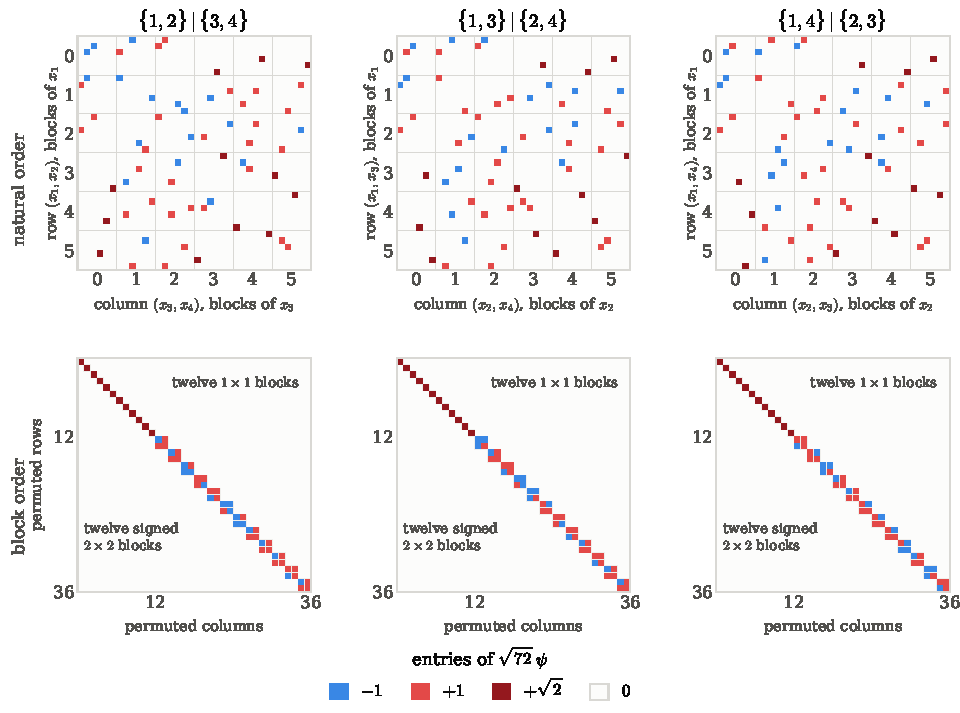
\includegraphics[width=\textwidth]{figures/amplitudes.pdf}
\caption{The three reshapings of $\sqrt{72}\,\psi$ for the bipartitions $12|34$, $13|24$ and $14|23$.  Top: natural
order.  Bottom: rows and columns permuted so that the twelve entries $\sqrt2$ form $1\times1$ blocks and the $48$
entries $\pm1$ form twelve $2\times2$ blocks, each proportional to an orthogonal matrix.}
\label{fig:amplitudes}
\end{figure*}

In the language of the officers~\cite{RBB22}, each row (and each column) of $O$ is the state of one officer.  In every
one of the three reshapings, $12$ officers are classical, i.e.\ product basis states $\ket{kl}$, and the remaining
$24$ are two-term states $(\ket{kl}\pm\ket{k'l'})/\sqrt2$ with $k\neq k'$ and $l\neq l'$: Bell-type states of rank and
regiment.  The twelve classical officers also show that $\ket\psi$ is as close to a product state as an AME$(4,6)$
state can be.  For any AME$(4,6)$ state, $|\langle abce|\psi\rangle|^2\le\langle ab|\rho_{12}|ab\rangle=1/36$, and
$\ket\psi$ attains this bound at the twelve basis states of $O$.

% =========================================================================================================
\section{Symmetry and linearization}\label{sec:symmetry}

The state was found by a search that uses only $N=4$ and $d=6$ as input.  We looked for AME states inside
eigenspaces of local symmetries $U^{\otimes4}$, $U=VDV^\dagger$, with $V$ Haar random and $D$ diagonal of finite
order; the spectra of $D$ were restricted by necessary conditions for an AME state to exist in the
eigenspace~\cite{repo}.  For $D=u=\mathrm{diag}(i,-1,-1,-i,-i,-i)$ and eigenvalue $-1$, the eigenspace of
$u^{\otimes4}$ is spanned by the $360$ basis states $\ket{x_1x_2x_3x_4}$ with $e_{x_1}+\dots+e_{x_4}\equiv2\pmod 4$,
where $e=(1,2,2,3,3,3)$.  A random-start optimization in this eigenspace finds AME states within a few
restarts~\cite{repo}.  The commutant of $u$, $U(1)\times U(2)\times U(3)$ on the levels $\{0\}$, $\{1,2\}$,
$\{3,4,5\}$, preserves the eigenspace.  Minimizing the number of non-zero coefficients over local frames in the
commutant, and then over all of $U(6)$, brought the state found to $72$ non-zero coefficients.  Their basis states
form an orthogonal array of strength $2$ and index $2$~\cite{HSS1999}: every pair of parties sees every pair of levels
exactly twice.

On such a support the AME conditions linearize.

\begin{lemma}\label{lem:blocks}
Let $S\subset\{0,\dots,5\}^4$ be such that, in each of the three bipartitions, the bipartite graph joining the
row and column labels of the points of $S$ has only components of size $1\times1$ and $2\times2$.  A state with
support exactly $S$ and coefficients $\sqrt{s_x/72}\,e^{i\varphi_x}$ is AME if and only if $s_x=2$ on every
$1\times1$ block and, on every $2\times2$ block
$\bigl(\begin{smallmatrix}a&b\\ c&e\end{smallmatrix}\bigr)$,
\begin{equation}\label{eq:congruence}
\begin{gathered}
s_a=s_e,\quad s_b=s_c,\quad s_a+s_b=2,\\
\varphi_a-\varphi_b-\varphi_c+\varphi_e\equiv\pi\pmod{2\pi}.
\end{gathered}
\end{equation}
In particular, there is a real AME state with support $S$ if and only if the congruences are solvable over
$\mathbb F_2$.
\end{lemma}

\begin{proof}
Each reshaping of $6\psi$ is a direct sum of its blocks, and it is unitary if and only if every block is.  A
$1\times1$ block is unitary if and only if its entry has modulus $1$.  A $2\times2$ block is unitary if and only if
its rows and columns have unit norm, which gives the three linear equations, and its two columns are orthogonal,
which, with all four entries non-zero, is the phase condition.  For phases in $\{0,\pi\}$ the congruences become
linear equations over $\mathbb F_2$.
\end{proof}

All $72$ points of the sparse support satisfy $\sum_j e_{x_j}\equiv2\pmod4$.  Every state supported there is
therefore an eigenvector of $u^{\otimes4}$ with eigenvalue $-1$.  This includes every state of the two families
below and, in particular, the real state $\ket\psi$.  The diagonal local unitaries that act on the support as a
scalar form, modulo phases on each party, the group $\mathbb Z_2\times\mathbb Z_2\times\mathbb Z_4$, and
$u^{\otimes4}$ is an element of order four in it.

% =========================================================================================================
\section{Two families through the real state}\label{sec:families}

Let $N$ be the twelve further basis states listed in Appendix~\ref{app:K}.  Like those of $O$, they have all labels
in $\{0,3,4,5\}$, exactly one of them $0$.  The $72$ states $L\cup O\cup N$ form the orthogonal array above.  In each
bipartition they split into $18$ blocks of size $2\times2$: the twelve $L$-blocks of $\ket\psi$, and six blocks with
two states of $O$ on one diagonal and two states of $N$ on the other.  Let $K\in\{0,\pm1\}^{72\times9}$ be the
integer matrix of Appendix~\ref{app:K} and $(K\theta)_x=\sum_jK_{xj}\theta_j$.  For $\delta\in[-1,1]$,
$\theta\in\mathbb R^9$ and $\sigma=\pm1$ define
\begin{multline}\label{eq:F72}
\ket{\psi_\sigma(\delta,\theta)}=\frac1{\sqrt{72}}\Big[\sum_{x\in L}\varepsilon_xe^{i(K\theta)_x}\ket x\\
+\sqrt{1+\delta}\sum_{x\in O}e^{i(K\theta)_x}\ket x\\
+i\sigma\sqrt{1-\delta}\sum_{x\in N}e^{i(K\theta)_x}\ket x\Big],
\end{multline}
and for $\theta\in\mathbb R^{11}$
\begin{multline}\label{eq:F60}
\ket{\psi_{\rm face}(\theta)}=\frac1{\sqrt{72}}\sum_{x\in L}\varepsilon_xe^{i(K'\theta)_x}\ket x\\
+\frac16\sum_{x\in O}e^{i(K'\theta)_x}\ket x ,
\end{multline}
where $K'$ is $K$ restricted to $L\cup O$, extended by two columns: $\theta_{10}$ acts on $\ket{3505}$ alone and
$\theta_{11}$ on $\ket{5045}$ alone.  Clearly $\ket\psi=\ket{\psi_{\rm face}(0)}=\ket{\psi_\pm(1,0)}$.

\begin{proposition}\label{prop:families}
(a) Every $\ket{\psi_\sigma(\delta,\theta)}$ is an AME$(4,6)$ state.  Up to diagonal local unitaries, every AME state
with support exactly $L\cup O\cup N$ is of this form with $|\delta|<1$.  The two values of $\sigma$ label the two
connected components of this set, which complex conjugation exchanges, and the family has $10$ parameters modulo
local unitaries.\\
(b) Every $\ket{\psi_{\rm face}(\theta)}$ is AME.  Up to diagonal local unitaries, every AME state with support
exactly $L\cup O$ is of this form; the moduli are rigid and the phases form one $11$-dimensional torus.\\
(c) $\ket{\psi_\sigma(1,\theta)}=\ket{\psi_{\rm face}(\theta,0,0)}$.  A state of the face is a limit of AME states
with support $L\cup O\cup N$ if and only if $\theta_{10},\theta_{11}\in2\pi\mathbb Z$.  Exactly eight such curves end
at $\ket\psi$, four in each component; they are $\delta\mapsto\ket{\psi_\sigma(\delta,\theta)}$ with $\theta$ from
Table~\ref{tab:branches}.\\
(d) No AME state with support exactly $L\cup O\cup N$ is real, even up to diagonal local unitaries.
\end{proposition}

\begin{proof}[Proof sketch]
All statements follow from Lemma~\ref{lem:blocks} by integer linear algebra.  On $L\cup O\cup N$ the moduli
equations have the one-parameter solution $s=1$ on $L$, $1+\delta$ on $O$ and $1-\delta$ on $N$.  The $54$
congruences have rank $42$; the real kernel, of dimension $30$, is spanned by the columns of $K$ and $21$
independent diagonal local phases.  Their Smith normal form has a single invariant factor $2$, so the solution set has two
components, containing the base points $\sigma=\pm1$.  On $L\cup O$ the states of $O$ are $1\times1$ blocks; the
$36$ remaining congruences have a $32$-dimensional kernel, spanned by $K'$ and the local phases, and all invariant
factors equal $1$.  For~(c), the $N$-phases of a limit must solve the $54$ congruences with the face phases fixed;
the solvability conditions involve only $\theta_{10}$ and $\theta_{11}$.  With the phases of $\ket\psi$ fixed, the
$54\times12$ system has invariant factors $1^92^3$, hence exactly eight solutions, all with phases $\pm\pi/2$.
Statement~(d) holds because the congruences on $L\cup O\cup N$ have no solution over $\mathbb F_2$.  The AME
property of Eqs.~\eqref{eq:F72} and~\eqref{eq:F60} for all parameters has also been checked symbolically~\cite{repo}.
\end{proof}

Each of the eight branches passes, at $\delta=0$, through a state with uniform amplitudes $1/\sqrt{72}$.  For
$\theta=0$ the coefficients are $\varepsilon_x$ on $L$, $1$ on $O$ and $i\sigma$ on $N$, so $W=\sqrt2\cdot6M$ has
entries in $\{0,\pm1,\pm i\}$, two per row and column, and $WW^\dagger=2\,\mathbb I$ in all three reshapings.  These
are two-unitary complex weighing matrices.  As $\delta$ increases to $1$, the weight of each entry of $N$ moves to
its partner in $O$, and the state stays AME until it becomes real at $\ket\psi$.

The first-order deformations of an AME state, modulo the tangent space of its local-unitary orbit, are a local-unitary
invariant.  Their dimension is $10$ for a generic member of~\eqref{eq:F72} and $11$ for a generic face state.  At
$\ket\psi$ it is $14$: $11$ directions along the face and $3$ spanned by the eight branches.  The real state is thus a
singular point at which the $11$-dimensional face and both $10$-dimensional components meet (Fig.~\ref{fig:families}).

\begin{figure*}[t]
\centering
\resizebox{0.9\textwidth}{!}{% Fig. 3 (input from main.tex): both faces, and both components joining the gluing loci C (delta = 1) and C' (delta = -1).
% Coordinates (x, depth, delta); the components bulge to depth -/+ b (1 - delta^2), front = F72^+, back = F72^-.
% The eight branches run from psi on C to the four real points of C' (up to diagonal local unitaries), one branch from
% each component to each point; the numbers are their classes (Theorem 1).  Dotted: path from the uniform state with
% four imaginary coefficients (in F72^+, delta = 0) to psi.
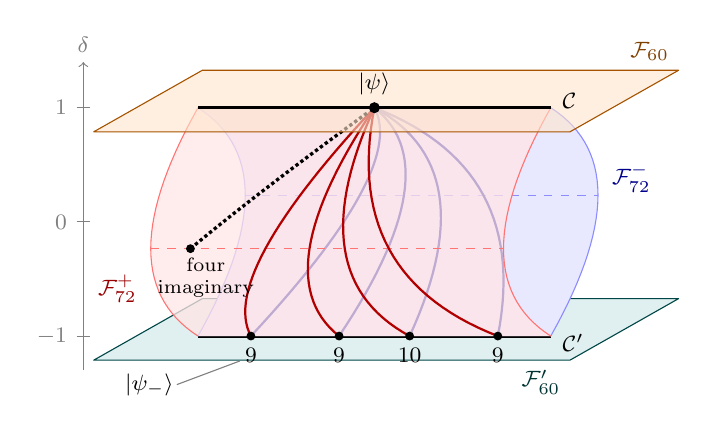
\begin{tikzpicture}[x={(0.56cm,0cm)},y={(0.30cm,0.17cm)},z={(0cm,1.45cm)},line join=round,font=\footnotesize]
  \def\b{2.0}
  \def\ends{1.2/9,3.2/9,4.8/10,6.8/9}
  % delta axis
  \draw[->,gray] (-2.6,0,-1.3) -- (-2.6,0,1.4) node[above] {$\delta$};
  \foreach \z in {1,0,-1} { \draw[gray] (-2.75,0,\z) -- (-2.45,0,\z) node[pos=0,left] {$\z$}; }
  % opposite face F60' and C'
  \fill[teal!12] (-1.4,-1.8,-1) -- (9.4,-1.8,-1) -- (9.4,2.8,-1) -- (-1.4,2.8,-1) -- cycle;
  \draw[teal!55!black] (-1.4,-1.8,-1) -- (9.4,-1.8,-1) -- (9.4,2.8,-1) -- (-1.4,2.8,-1) -- cycle;
  \node[teal!40!black,anchor=north east] at (9.4,-1.8,-1) {$\mathcal F_{60}'$};
  \draw[very thick] (0,0,-1) -- (8,0,-1);
  \node[anchor=west] at (8.05,0,-1.06) {$\mathcal C'$};
  % back component F72^-
  \fill[blue!9] plot[domain=1:-1,variable=\t,samples=31] (8,{\b*(1-\t*\t)},\t)
                -- plot[domain=-1:1,variable=\t,samples=31] (0,{\b*(1-\t*\t)},\t) -- cycle;
  \foreach \xx in {0,8} { \draw[blue!45] plot[domain=-1:1,variable=\t,samples=31] (\xx,{\b*(1-\t*\t)},\t); }
  \draw[blue!45,dashed] (0,\b,0) -- (8,\b,0);
  \foreach \e/\c in \ends { \draw[blue!60!black,thick] plot[domain=1:-1,variable=\t,samples=31]
                             ({4+(\e-4)*(1-\t)/2},{\b*(1-\t*\t)},\t); }
  \node[blue!55!black,anchor=west] at (8.1,\b,0.15) {$\mathcal F_{72}^-$};
  % front component F72^+
  \fill[red!10,opacity=0.75] plot[domain=1:-1,variable=\t,samples=31] (8,{-\b*(1-\t*\t)},\t)
                -- plot[domain=-1:1,variable=\t,samples=31] (0,{-\b*(1-\t*\t)},\t) -- cycle;
  \foreach \xx in {0,8} { \draw[red!55] plot[domain=-1:1,variable=\t,samples=31] (\xx,{-\b*(1-\t*\t)},\t); }
  \draw[red!55,dashed] (0,-\b,0) -- (8,-\b,0);
  \foreach \e/\c in \ends { \draw[red!70!black,thick] plot[domain=1:-1,variable=\t,samples=31]
                             ({4+(\e-4)*(1-\t)/2},{-\b*(1-\t*\t)},\t); }
  \node[red!60!black,anchor=east] at (-0.1,-\b,-0.35) {$\mathcal F_{72}^+$};
  % the uniform state with four imaginary coefficients and the path to psi
  \draw[densely dotted,very thick] plot[domain=0:0.97,variable=\t,samples=21] ({0.9+3.1*\t},{-\b*(1-\t*\t)},\t);
  \fill (0.9,-\b,0) circle (1.6pt);
  \node[anchor=north,align=center,font=\scriptsize,inner sep=1pt] at (1.25,-\b,-0.05) {four\\imaginary};
  % face F60 and C (drawn last: seen from above, it covers the top of the front component)
  \fill[orange!20,opacity=0.6] (-1.4,-1.8,1) -- (9.4,-1.8,1) -- (9.4,2.8,1) -- (-1.4,2.8,1) -- cycle;
  \draw[orange!65!black] (-1.4,-1.8,1) -- (9.4,-1.8,1) -- (9.4,2.8,1) -- (-1.4,2.8,1) -- cycle;
  \node[orange!50!black,anchor=south east] at (9.4,2.8,1) {$\mathcal F_{60}$};
  \draw[very thick] (0,0,1) -- (8,0,1);
  \node[anchor=west] at (8.05,0,1.06) {$\mathcal C$};
  % the real states
  \fill (4,0,1) circle (2pt) node[above=1pt] {$\ket\psi$};
  \foreach \e/\c in \ends { \fill (\e,0,-1) circle (1.6pt) node[below=1pt] {$\c$}; }
  \draw[gray] ([xshift=-4pt,yshift=-9pt]1.2,0,-1) -- ++(-0.8cm,-0.3cm) node[left,black,inner sep=1pt] {$\ket{\psi_-}$};
\end{tikzpicture}
}
\caption{The families of Proposition~\ref{prop:families}.  The face $\mathcal F_{60}$ (top) is an $11$-dimensional
phase torus.  The two components $\mathcal F_{72}^\pm$ ($\sigma=\pm1$, complex conjugate to each other) are
$10$-dimensional and attach to the face along the $9$-torus $\mathcal C=\{\theta_{10}=\theta_{11}=0\}$; $\delta$ runs
vertically.  Eight straight branches start at the real state $\ket\psi\in\mathcal C$ and cross the
uniform-amplitude slice $\delta=0$.}
\label{fig:families}
\end{figure*}

% =========================================================================================================
\section{Classification of the real states}\label{sec:real}

By Lemma~\ref{lem:blocks}, a real state with support exactly $L\cup O$ is determined by signs that solve the $36$
congruences over $\mathbb F_2$.  There are $2^{32}$ such sign patterns.  Modulo diagonal local unitaries they give
exactly $2048$ distinct real AME states, of which $512$ lie on $\mathcal C$ and are limits of the support-$72$
family.  Flipping the sign of any coefficient $1/6$ keeps a state AME, since these are $1\times1$ blocks.  The level
relabellings and party permutations that preserve $L\cup O$ form a group of order $192$, which has $16$ orbits on
the $2048$ states, eight of size $64$ and eight of size $192$.

\begin{theorem}\label{thm:classes}
The $2048$ real AME$(4,6)$ states with support $L\cup O$ fall into exactly eight classes under local unitaries and
permutations of the parties.  The representatives are listed in Table~\ref{tab:classes}.
\end{theorem}

\begin{proof}
\emph{At most eight.}  States in one orbit are related by monomial local unitaries and party permutations.  The
orbits pair up: within each pair, the real local orthogonal map $H_{12}^{\otimes4}$, a $2\times2$ Hadamard rotation on
the levels $\{1,2\}$ of every party, followed by a monomial map, takes one orbit to the other~\cite{repo}.\\
\emph{At least eight.}  Let $J$ be the real Jacobian of the map $\psi\mapsto(\rho_A)_{|A|=2}$ to all six
two-party marginals, and $N(t)$ the number of eigenvalues of $72J^{T}J$ below $t$.  A local unitary acts orthogonally
on the state and on each marginal; a party permutation permutes the marginals.  The spectrum of $J^TJ$, and so
$N(t)$, is therefore invariant under both.  The values $N(41/8)$ on the eight representatives are pairwise different
(Table~\ref{tab:classes}).  We certify them rigorously.  $72J^TJ$ has entries in $\mathbb Z[\sqrt2]$ and splits into
blocks of size at most $160$.  For each block $G$ we form $X=V^T(G-t\mathbb I)V$ in ball arithmetic~\cite{Arb2017},
with $V$ its numerical eigenvectors, and check that every Gershgorin interval of $X$ excludes $0$.  By Sylvester's law
of inertia, the number of negative intervals then equals the number of eigenvalues of $G$ below $t$.
\end{proof}

\begin{table}[t]
\caption{The eight classes of Theorem~\ref{thm:classes}.  Representative: $\ket\psi$ with the listed coefficients
$1/6$ negated.  ``On $\mathcal C$'': limits of the support-$72$ family.  Dim: first-order deformations modulo local
unitaries.  $N(41/8)$: the certified invariant of the proof.}
\label{tab:classes}
\begin{ruledtabular}
\begin{tabular}{clcccc}
class & flipped & states & on $\mathcal C$ & dim & $N(41/8)$\\
\hline
1 & -- & $128$ & yes & $14$ & $261$\\
2 & $0344$, $3505$ & $384$ & yes & $14$ & $265$\\
3 & $5303$ & $128$ & no & $11$ & $255$\\
4 & $5430$ & $128$ & no & $11$ & $256$\\
5 & $5045$ & $128$ & no & $11$ & $264$\\
6 & $0533$ & $384$ & no & $11$ & $254$\\
7 & $0455$ & $384$ & no & $11$ & $257$\\
8 & $0344$ & $384$ & no & $11$ & $258$
\end{tabular}
\end{ruledtabular}
\end{table}

Simpler invariants do not separate the classes: all polynomial local-unitary invariants of degree four that we
evaluated, and the power traces $\mathrm{Tr}(J^TJ)^k$ for $k\le8$, take equal values on classes $3$--$8$.

The real states are isolated: no continuous family of real AME states passes through any of them, modulo local
orthogonal maps.  For $14$ of the $16$ orbits there is no real first-order deformation.  For the two orbits of
class~2 the two real first-order deformations are obstructed at second order (numerical)~\cite{repo}.  Within the
families of Sec.~\ref{sec:families} the real states are therefore isolated points of complex continua.

The deformation dimensions also separate our states from the known solutions.  They are $14$ and $11$ for the real
classes and $10$ for the support-$72$ family, but $4$ for the golden state of Ref.~\cite{RBB22} and $3$ for the
two-unitary Hadamard matrix $H(0)$ of Ref.~\cite{BZ24}.  None of our states is therefore locally equivalent to those
(numerical rank decisions, with gaps of $10^{-15}$ against $10^{-2}$).

% =========================================================================================================
\section{Discussion}\label{sec:discussion}

The real states have $60$ non-zero coefficients.  The golden state has $112$~\cite{RBB22}, the sparsest previously
reported, and an entropy-optimal form of it has $144$~\cite{Ram25}.  A lower bound for the support of any AME$(4,6)$
state follows from the argument used above.  A coefficient of modulus $1/6$ exhausts the norm of its row and column
in every reshaping, so these classical officers form a code of length $4$ and minimum distance $3$ over six symbols,
with at most $34$ codewords~\todo{ref for $A_6(4,3)=34$}.  Every other row needs at least two entries, so the support
is at least $72-t\ge38$, where $t$ is the number of classical officers.  Whether the gap between $38$ and $60$ can be
closed is open.

Further questions remain.  Are there real AME$(4,6)$ states outside the families found here, and do the real states
admit a form with all amplitudes of modulus $1/36$, i.e.\ a real-equivalent two-unitary Hadamard matrix?  Any such
form would have to preserve the twelve product states of maximal overlap $1/6$.  The eigenspace of $u^{\otimes4}$ also
contains AME states outside these families: about one in eight search hits lies on a three-parameter family of
complex AME states with $348$ of the $360$ coefficients non-zero and deformation dimension $3$, which we did not
manage to bring to a sparse or a real form (numerical).  Whether it is related to the Hadamard family of
Ref.~\cite{BZ24} is open.  Finally, a real two-unitary
of order $36$ is a real perfect tensor, which can serve as a real dual-unitary gate or as the building block of a
holographic code with real amplitudes~\cite{PYHP2015,BKP2019}.

\begin{acknowledgments}
\todo{Acknowledgments.}
\end{acknowledgments}

\paragraph*{Data and code availability.}  The state, the families, the class representatives and scripts verifying
every statement of this paper are available in Ref.~\cite{repo}.

\onecolumngrid
\appendix
\section{Block decomposition of the three reshapings}\label{app:blocks}
Labels are pairs of levels in the order of the parties of the bipartition; entries are those of $O=6M$.  Each
$2\times2$ block is $1/\sqrt2$ times the sign matrix shown.
\paragraph{Pairing $\{1,2\}|\{3,4\}$.}
$1\times1$ blocks (row$\to$column, entry $1$): $03\to44$, $04\to55$, $05\to33$, $30\to34$, $33\to50$, $35\to05$, $40\to53$, $44\to04$, $45\to40$, $50\to45$, $53\to03$, $54\to30$.

$2\times2$ blocks (rows; columns; sign matrix):
\begin{center}\small\begin{tabular}{llll}
$00,55$; $12,21$; $\left(\begin{smallmatrix}-&+\\+&+\end{smallmatrix}\right)$ & $01,20$; $02,20$; $\left(\begin{smallmatrix}-&+\\+&+\end{smallmatrix}\right)$ & $02,10$; $01,10$; $\left(\begin{smallmatrix}-&+\\-&-\end{smallmatrix}\right)$ & $11,22$; $00,54$; $\left(\begin{smallmatrix}+&+\\+&-\end{smallmatrix}\right)$ \\
$12,21$; $35,43$; $\left(\begin{smallmatrix}+&+\\-&+\end{smallmatrix}\right)$ & $13,41$; $15,32$; $\left(\begin{smallmatrix}-&-\\+&-\end{smallmatrix}\right)$ & $14,31$; $23,41$; $\left(\begin{smallmatrix}-&+\\-&-\end{smallmatrix}\right)$ & $15,52$; $24,52$; $\left(\begin{smallmatrix}-&+\\+&+\end{smallmatrix}\right)$ \\
$23,42$; $25,31$; $\left(\begin{smallmatrix}-&+\\+&+\end{smallmatrix}\right)$ & $24,32$; $13,42$; $\left(\begin{smallmatrix}-&+\\+&+\end{smallmatrix}\right)$ & $25,51$; $14,51$; $\left(\begin{smallmatrix}+&+\\-&+\end{smallmatrix}\right)$ & $34,43$; $11,22$; $\left(\begin{smallmatrix}-&+\\+&+\end{smallmatrix}\right)$ \\
\end{tabular}\end{center}

\paragraph{Pairing $\{1,3\}|\{2,4\}$.}
$1\times1$ blocks (row$\to$column, entry $1$): $03\to53$, $04\to34$, $05\to45$, $30\to55$, $33\to04$, $35\to30$, $40\to44$, $44\to50$, $45\to03$, $50\to33$, $53\to40$, $54\to05$.

$2\times2$ blocks (rows; columns; sign matrix):
\begin{center}\small\begin{tabular}{llll}
$00,43$; $12,21$; $\left(\begin{smallmatrix}-&-\\-&+\end{smallmatrix}\right)$ & $01,20$; $02,20$; $\left(\begin{smallmatrix}-&+\\+&+\end{smallmatrix}\right)$ & $02,10$; $01,10$; $\left(\begin{smallmatrix}+&+\\-&+\end{smallmatrix}\right)$ & $11,22$; $00,35$; $\left(\begin{smallmatrix}-&-\\+&-\end{smallmatrix}\right)$ \\
$12,21$; $43,54$; $\left(\begin{smallmatrix}-&-\\-&+\end{smallmatrix}\right)$ & $13,42$; $25,32$; $\left(\begin{smallmatrix}+&-\\+&+\end{smallmatrix}\right)$ & $14,31$; $23,41$; $\left(\begin{smallmatrix}+&+\\+&-\end{smallmatrix}\right)$ & $15,51$; $14,52$; $\left(\begin{smallmatrix}+&+\\-&+\end{smallmatrix}\right)$ \\
$23,41$; $15,31$; $\left(\begin{smallmatrix}-&+\\+&+\end{smallmatrix}\right)$ & $24,32$; $13,42$; $\left(\begin{smallmatrix}+&+\\-&+\end{smallmatrix}\right)$ & $25,52$; $24,51$; $\left(\begin{smallmatrix}-&+\\+&+\end{smallmatrix}\right)$ & $34,55$; $11,22$; $\left(\begin{smallmatrix}-&+\\+&+\end{smallmatrix}\right)$ \\
\end{tabular}\end{center}

\paragraph{Pairing $\{1,4\}|\{2,3\}$.}
$1\times1$ blocks (row$\to$column, entry $1$): $03\to53$, $04\to34$, $05\to45$, $30\to35$, $34\to03$, $35\to50$, $40\to54$, $43\to05$, $44\to40$, $50\to43$, $53\to30$, $55\to04$.

$2\times2$ blocks (rows; columns; sign matrix):
\begin{center}\small\begin{tabular}{llll}
$00,33$; $12,21$; $\left(\begin{smallmatrix}+&+\\-&+\end{smallmatrix}\right)$ & $01,20$; $02,20$; $\left(\begin{smallmatrix}+&-\\+&+\end{smallmatrix}\right)$ & $02,10$; $01,10$; $\left(\begin{smallmatrix}-&-\\-&+\end{smallmatrix}\right)$ & $11,22$; $00,44$; $\left(\begin{smallmatrix}-&+\\+&+\end{smallmatrix}\right)$ \\
$12,21$; $33,55$; $\left(\begin{smallmatrix}-&+\\+&+\end{smallmatrix}\right)$ & $13,32$; $24,42$; $\left(\begin{smallmatrix}+&-\\+&+\end{smallmatrix}\right)$ & $14,51$; $15,52$; $\left(\begin{smallmatrix}+&-\\+&+\end{smallmatrix}\right)$ & $15,41$; $23,31$; $\left(\begin{smallmatrix}+&-\\+&+\end{smallmatrix}\right)$ \\
$23,31$; $14,41$; $\left(\begin{smallmatrix}+&-\\-&-\end{smallmatrix}\right)$ & $24,52$; $25,51$; $\left(\begin{smallmatrix}-&+\\+&+\end{smallmatrix}\right)$ & $25,42$; $13,32$; $\left(\begin{smallmatrix}-&-\\-&+\end{smallmatrix}\right)$ & $45,54$; $11,22$; $\left(\begin{smallmatrix}+&+\\-&+\end{smallmatrix}\right)$ \\
\end{tabular}\end{center}


\section{Phase directions and branches}\label{app:K}
The sets $O$ and $N$ are
\begin{aligned}
P_1&=\{0344,3505,4053,5430\},\\
P_2&=\{0455,3034,4540,5303\},\\
P_3&=\{0533,3350,4404,5045\},\\
P'_1&=\{0353,3530,4044,5405\},\\
P'_2&=\{0434,3055,4503,5340\},\\
P'_3&=\{0545,3304,4450,5033\}.
\end{aligned}

The columns of $K$ are listed in Table~\ref{tab:K}, the branches through $\ket\psi$ in Table~\ref{tab:branches}.

\begin{table}[h]
\caption{The phase directions: $\theta_j$ multiplies the listed basis states by $e^{\pm i\theta_j}$; superscripts
mark states of $O$ and $N$, unmarked states are in $L$.  On the face, $\theta_{10}$ acts on $\ket{3505}$ alone and
$\theta_{11}$ on $\ket{5045}$ alone.}
\label{tab:K}
\begin{center}\small\begin{tabular}{lll}
\hline
angle & phase $e^{+i\theta_j}$ on & phase $e^{-i\theta_j}$ on\\
\hline
$\theta_{1}$ & $0102,\ 0201$ & $1010,\ 2020$\\
$\theta_{2}$ & $1332,\ 2331$ & $4115,\ 4225$\\
$\theta_{3}$ & $1423,\ 2413$ & $3141,\ 3242$\\
$\theta_{4}$ & $0344^{\scriptscriptstyle O},\ 0545^{\scriptscriptstyle O'},\ 4044^{\scriptscriptstyle O'},\ 4540^{\scriptscriptstyle O},\ 5045^{\scriptscriptstyle O},\ 5340^{\scriptscriptstyle O'}$ & --\\
$\theta_{5}$ & $0353^{\scriptscriptstyle O'},\ 0533^{\scriptscriptstyle O},\ 4053^{\scriptscriptstyle O},\ 4503^{\scriptscriptstyle O'},\ 5033^{\scriptscriptstyle O'},\ 5303^{\scriptscriptstyle O}$ & --\\
$\theta_{6}$ & $0344^{\scriptscriptstyle O},\ 0353^{\scriptscriptstyle O'},\ 0434^{\scriptscriptstyle O'},\ 0455^{\scriptscriptstyle O},\ 0533^{\scriptscriptstyle O},\ 0545^{\scriptscriptstyle O'}$ & --\\
$\theta_{7}$ & $3350^{\scriptscriptstyle O},\ 3530^{\scriptscriptstyle O'},\ 4450^{\scriptscriptstyle O'},\ 4540^{\scriptscriptstyle O},\ 5340^{\scriptscriptstyle O'},\ 5430^{\scriptscriptstyle O}$ & --\\
$\theta_{8}$ & $0533^{\scriptscriptstyle O},\ 0545^{\scriptscriptstyle O'},\ 3505^{\scriptscriptstyle O},\ 3530^{\scriptscriptstyle O'},\ 4503^{\scriptscriptstyle O'},\ 4540^{\scriptscriptstyle O}$ & --\\
$\theta_{9}$ & $5033^{\scriptscriptstyle O'},\ 5045^{\scriptscriptstyle O},\ 5303^{\scriptscriptstyle O},\ 5340^{\scriptscriptstyle O'},\ 5405^{\scriptscriptstyle O'},\ 5430^{\scriptscriptstyle O}$ & --\\
\hline
\end{tabular}\end{center}

\end{table}

\begin{table}[h]
\caption{The eight branches $\delta\mapsto\ket{\psi_\sigma(\delta,\theta)}$ that end at $\ket\psi$ ($\delta=1$), up to
diagonal local phases; the four values of $\theta$ form a group $\mathbb Z_2\times\mathbb Z_2$.}
\label{tab:branches}
\begin{center}\small\begin{tabular}{ll}
\hline
$\theta$ & $\sigma$\\
\hline
$0$ & $+1,-1$\\
$\pi(0,1,1,0,0,0,0,1,1)$ & $+1,-1$\\
$\pi(1,0,1,1,1,0,0,1,1)$ & $+1,-1$\\
$\pi(1,1,0,1,1,0,0,0,0)$ & $+1,-1$\\
\hline
\end{tabular}\end{center}

\end{table}
\clearpage

\twocolumngrid
\bibliography{references}
\end{document}
